\documentclass{report}
\setlength{\parskip}{0pt} % esp. entre parrafos
\setlength{\parindent}{20pt} % esp. al inicio de un parrafo
\usepackage{amsmath} % mates
\usepackage{listings}
\usepackage{xcolor}
\usepackage[sort&compress,numbers]{natbib} % referencias
\usepackage{url} % que las URLs se vean lindas
\usepackage[top=10mm,left=20mm,right=20mm,bottom=25mm]{geometry} % \textbf{\textbf{}}margenes
\usepackage{hyperref} % ligas de URLs
\usepackage{graphicx} % poner figuras
\usepackage{caption}
\usepackage{subcaption}
\usepackage[spanish]{babel} % otros idiomas
\hypersetup{
    colorlinks=true,
    linkcolor=blue,
    filecolor=blue,      
    urlcolor=blue,
}
\renewcommand{\lstlistingname}{C\'odigo}
\definecolor{codegreen}{rgb}{0,0.6,0}
\definecolor{codegray}{rgb}{0.5,0.5,0.5}
\definecolor{codepurple}{rgb}{0.58,0,0.82}
\definecolor{backcolour}{rgb}{0.95,0.95,0.92}
\lstdefinestyle{mystyle}{
    backgroundcolor=\color{backcolour},   
    commentstyle=\color{codegreen},
    keywordstyle=\color{magenta},
    numberstyle=\tiny\color{codegray},
    stringstyle=\color{codepurple},
    basicstyle=\ttfamily\footnotesize,
    breakatwhitespace=false,         
    breaklines=true,                 
    keepspaces=true,                 
    numbers=left,                    
    numbersep=5pt,                  
    showspaces=false,                
    showstringspaces=false,
    showtabs=false,                  
    tabsize=2
}
\lstset{style=mystyle}

\title{Reporte 5:\\M\'etodo Monte-Carlo}
\author{Jorge Torres}
\date{\today}

\begin{document}
\maketitle

\chapter{Estimaci\'on de una Integral Definida}

\section{Objetivo}
El objetivo de esta actividad es el estudiar estadísticamente la convergencia de la precisión del estimado de una integral definida (ecuaci\'on \ref{eq1}), con el método Monte Carlo, compar\'andolo con el valor producido por \href{https://www.wolframalpha.com/input?i=integrate+1%2F%28exp%28x%29%2Bexp%28-x%29%29+from+3+to+7}{Wolfram Alpha}, en términos de 1) el error absoluto, 2) el error cuadrado y 3) la cantidad de decimales correctos, aumentando el tamaño de muestra en tres niveles.

\begin{equation}\label{eq1}
    \int_{3}^{7} \frac{1}{\exp{(x)} + \exp{(-x)}} \,dx
\end{equation}

\section{Desarrollo}
El desarrollo de la actividad est\'a basado en el \href{https://github.com/satuelisa/Simulation/blob/master/MonteCarlo/integral.py}{c\'odigo} implementado por E. Schaeffer \cite{elisa1}. En el c\'odigo \ref{codigo1} se establecen los par\'ametros para la ejecuci\'on del programa, que consisten en 1) el valor estimado por Wolfram Alpha, \texttt{wolfram}, 2) el rango en que se define la integral, \texttt{desde} y \texttt{hasta}, 3) la cantidad de n\'umeros pseudoaleatorios que se producen con la distribuci\'on definida por la integral, \texttt{pedazo}, y 4) la lista de niveles en que se var\'ia la cantidad de iteraciones del experimento, \texttt{cuantos}.

\begin{lstlisting}[caption=Par\'ametros, label=codigo1, language=Python]
wolfram = 0.048834111126049311
desde = 3
hasta = 7
pedazo = 50000
cuantos = [500, 5000, 50000]
\end{lstlisting}

Se define la normalizaci\'on de la integral por medio de la funci\'on \texttt{g(x)} dada por la ecuaci\'on \ref{eq2} y se vectoriza la distribuci\'on resultante en el c\'odigo \ref{codigo2}.

\begin{equation}\label{eq2}
    \frac{2}{\pi}\int_{-\infty}^{\infty} \frac{1}{\exp{(x)} + \exp{(-x)}} \,dx
\end{equation}

\begin{lstlisting}[caption=Normalizaci\'on de la Integral, label=codigo2, language=Python]
def g(x):
    return (2  / (pi * (exp(x) + exp(-x))))

vg = np.vectorize(g)
X = np.arange(-8, 8, 0.05)
Y = vg(X
\end{lstlisting}

Importando una \href{https://github.com/satuelisa/Simulation/blob/master/MonteCarlo/GeneralRandom.py}{receta} y utiliz\'andola en conjunto con la funci\'on \texttt{parte()} del c\'odigo \ref{codigo3}, se genera una cantidad de n\'umeros aleatorios con una distribuci\'on de acuerdo a la integral normalizada, visualizada en la figura \ref{fig1}.

\begin{lstlisting}[caption= Generaci\'on de N\'umeros Aleatorios, label=codigo3, language=Python]
generador = GeneralRandom(np.asarray(X), np.asarray(Y))

def parte(replica):
    V = generador.random(pedazo)[0]
    return ((V >= desde) & (V <= hasta)).sum()
\end{lstlisting}

\begin{figure}[h!]
    \centering
    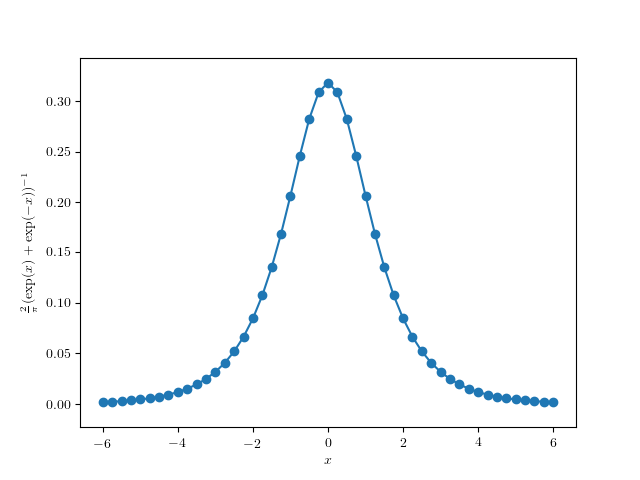
\includegraphics[width=\textwidth]{images/IntNorm.png}
    \caption{Distribuci\'on de la integral normalizada. Obtenida de \href{https://satuelisa.github.io/simulation/p5.html}{P5 - Simulaci\'on}}
    \label{fig1}
\end{figure}

Para determinar la cantidad de decimales correctos entre el estimado de la integral y el valor de Wolfram Alpha, se define la funci\'on \texttt{compare\_strings} en el c\'odigo \ref{codigo4}, que compara ambos valores caracter por caracter hasta que el decimal es diferente.

\begin{lstlisting}[caption= Comparaci\'on de Decimales, label=codigo4, language=Python]
def compare_strings(a, b):
    a = str(a)
    b = str(b)
    
    if a is None or b is None:
        return 0
    
    size = min(len(a), len(b))
    count = 0

    for i in range(size):
        if a[i] == b[i]:
            count += 1
        else:
            break
    return count
\end{lstlisting}

Por \'ultimo, por medio del c\'odigo \ref{codigo5} se ejecutan las iteraciones del experimento y se calculan los valores de los errores para poder comparar las estimaciones de la integral definida dependiendo de la cantidad de iteraciones. El desarrollo completo del c\'odigo se puede revisar en el \href{https://github.com/FeroxDeitas/Simulacion-Nano/tree/main/Tareas/P5}{repositorio} en GitHub de J. Torres \cite{jorge1}.

\begin{lstlisting}[caption= Estimaci\'on de la Integral y C\'alculo de Errores, label=codigo5, language=Python]
if __name__ == "__main__":
    with multiprocessing.Pool() as pool:
        for c in cuantos:
            p = c * pedazo
            puntos.append('{:.1e}'.format(p))
            montecarlo = pool.map(parte, range(c))
            integral = sum(montecarlo) / p
            valor = (pi / 2) * integral
            ae.append(abs(valor - wolfram))
            se.append(((valor - wolfram)**2))
            dec.append(compare_strings(wolfram, valor) - 2)
        resultados = {'Iteraciones': puntos,
                      'Error Absoluto': ae,
                      'Error Cuadrado': se,
                      'Decimales Correctos': dec}
        df = pd.DataFrame(resultados)
\end{lstlisting}

\section{Resultados}\label{res}
En los diagramas de la figura \ref{errores} se puede apreciar la variaci\'on en los valores de error absoluto (figura \ref{errabs}), error cuadrado (figura \ref{errcua}), y cantidad de decimales correctos (figura \ref{decimal}), al comparar entre los valores de la integral definida estimados por Wolfram Alpha y por el c\'odigo desarrollado en la actividad.

\begin{figure}[h]
     \centering
     \begin{subfigure}[b]{0.49\textwidth}
         \centering
         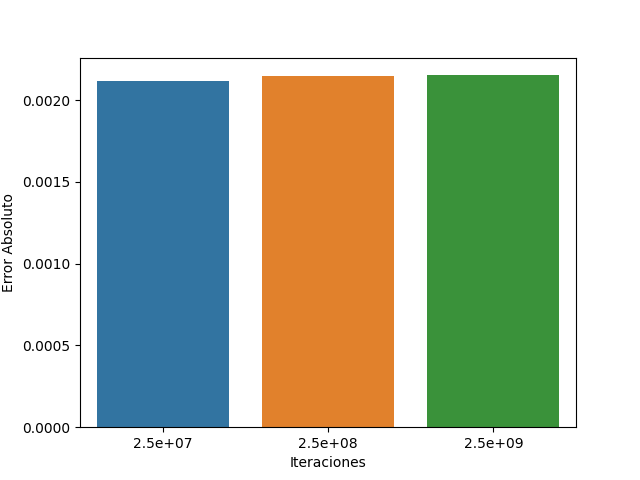
\includegraphics[width=\textwidth]{images/AbsErr.png}
         \caption{Error absoluto.}
         \label{errabs}
     \end{subfigure}
     \begin{subfigure}[b]{0.49\textwidth}
         \centering
         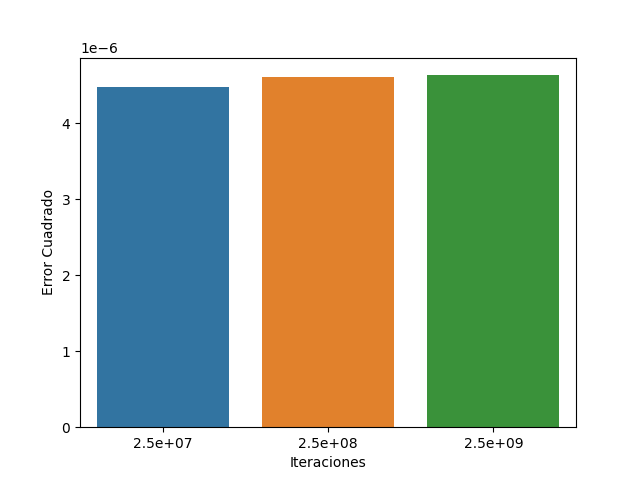
\includegraphics[width=\textwidth]{images/SqErr.png}
         \caption{Error cuadrado.}
         \label{errcua}
     \end{subfigure}
     \begin{subfigure}[b]{0.49\textwidth}
         \centering
         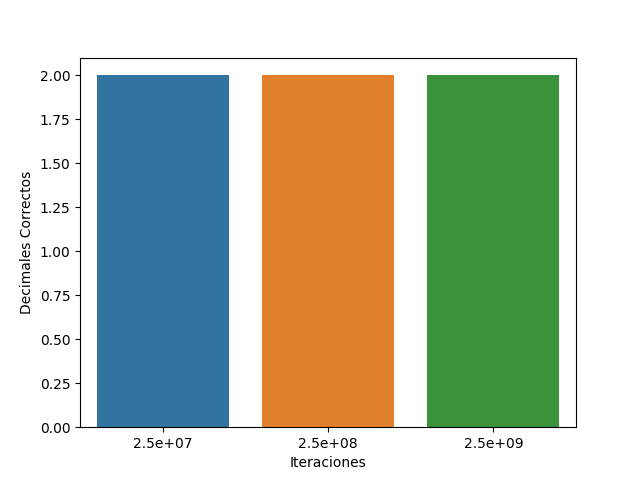
\includegraphics[width=\textwidth]{images/Decimals.png}
         \caption{Decimales correctos.}
         \label{decimal}
     \end{subfigure}
     \caption{Errores determinados entre la estimaci\'on de Wolfram Alpha y la calculada por el c\'odigo desarrollado.}
     \label{errores}
\end{figure}

\section{Conclusiones}
Como se puede apreciar en los diagramas de la secci\'on \ref{res}, aumentar la cantidad de iteraciones de $2.5\times10^7$ hasta $2.5\times10^9$ no presenta una diferencia apreciable en ning\'un tipo de error. Lo que es m\'as, tanto el error absoluto como el error cuadrado son m\'inimos y no representar\'ian un error estrictamente significativo. Sin embargo, se puede ver que la cantidad de decimales correctos no excede un m\'aximo de dos, por lo que el rango de error comienza a crecer en las mil\'esimas. En muchas aplicaciones, este rango podr\'ia causar diferencias bastante apreciables en c\'alculos que impliquen m\'as precisi\'on.

\chapter{Estimaci\'on de $\pi$}

\section{Objetivo}
El primer reto de esta actividad consiste en utilizar el m\'etodo Monte-Carlo para estimar el valor de $\pi$ a partir de una serie de puntos, determinando si las coordenadas de estos puntos se encuentran dentro o fuera del \'area de un c\'irculo de radio $r$.

\section{Desarrollo}
El c\'odigo \ref{codigo6} es tomado directamente del m\'etodo descrito por W. Kurt \cite{kurt1}, y en \'el se utiliza la relaci\'on entre el \'area de un c\'irculo y el cuadrado que lo circunscribe para aproximar el valor de $pi$ a partir de una serie de puntos de n\'umeros generados aleatoriamente dentro de una distribuci\'on normal. M\'as espec\'ificamente, se suma la cantidad de puntos que queda dentro del c\'irculo, se divide entre la cantidad total de puntos, y se multiplica por $4$ para obtener la aproximaci\'on.

\begin{lstlisting}[caption= C\'alculo de $\pi$ por M\'etodo Monte-Carlo, label=codigo6, language=R]
runs <- 1000000
xs <- runif(runs,min=-0.5,max=0.5)
ys <- runif(runs,min=-0.5,max=0.5)
in.circle <- xs^2 + ys^2 <= 0.5^2
mc.pi <- (sum(in.circle)/runs)*4)
plot(xs,ys,pch='.',col=ifelse(in.circle,"blue","grey")
     ,xlab='',ylab='',asp=1,
     main=paste("MC Approximation of Pi =",mc.pi))
\end{lstlisting}

\section{Resultados}
En la figura \ref{fig2} se visualiza de manera clara la serie de puntos ubicados aleatoriamente, que caen tanto dentro como fuera del c\'irculo. Tambi\'en se puede apreciar la aproximaci\'on calculada, $\pi=3.141956$.

\begin{figure}
    \centering
    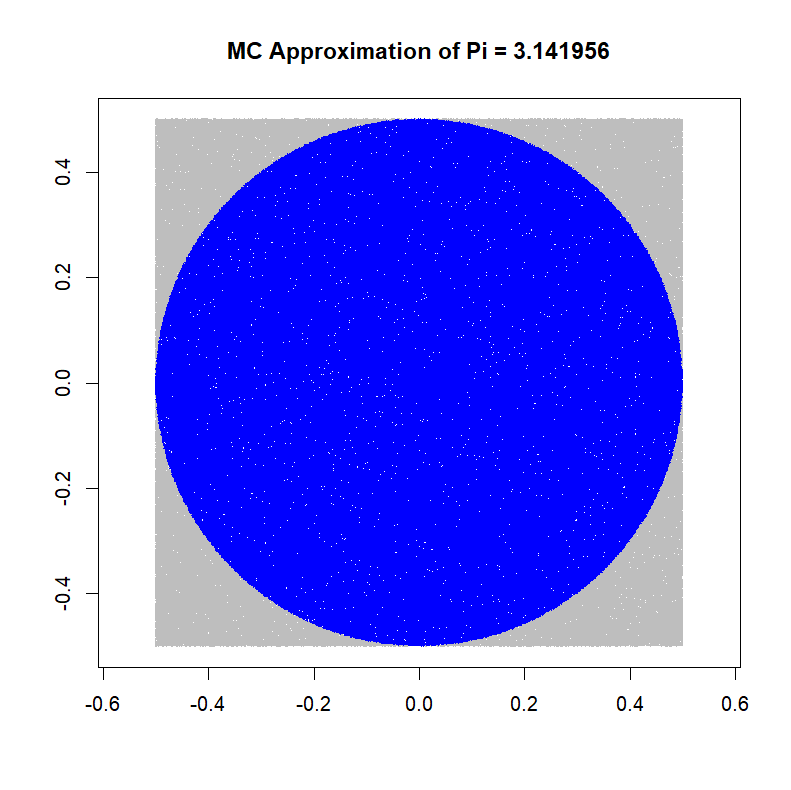
\includegraphics[width=\textwidth]{images/circulo.png}
    \caption{C\'irculo formado por los puntos aleatorios.}
    \label{fig2}
\end{figure}

\section{Conclusiones}
Inmediatamente queda claro que \'este m\'etodo es \'util para aproximar valores de procesos que son complejos de calcular anal\'iticamente con una precisi\'on aceptable, ya que se ha podido estimar $\pi$ correctamente en un rango tres decimales. Es de esperar que la precisi\'on aumente con la cantidad de puntos que se generan, pero en esta actividad no se han realizado pruebas para confirmarlo.

\bibliography{tarea_5}
\bibliographystyle{plainnat}

\end{document}
